\section{Results: A Reproducible Writer Meets Semantic Competition}
\label{sec:results}

\subsection{A non-generic write effect reproduces}
\label{sec:qwen-replication}

\begin{table}[H]
\centering
\caption{Controlled decodability of clinical concepts at the final visual block.}
\label{tab:decoding}
\resizebox{\ifdim\width>\linewidth\linewidth\else\width\fi}{!}{%
\begin{tabular}{lllccc}
\toprule
Model & Concept & Locus & \shortstack{AUROC \\ {[95\% CI]}} & \shortstack{Control mean \\ {(5--95\%)}} & \shortstack{Selectivity \\ {[95\% CI]}} \\
\midrule
LLaVA-1.5-7B & Effusion & CLIP L22 & \shortstack{0.7788 \\ \mbox{[0.7538, 0.8031]}} & \shortstack{0.6649 \\ \mbox{(0.5750--0.7450)}} & \shortstack{0.1139 \\ \mbox{[0.0875, 0.1404]}} \\
LLaVA-1.5-7B & Edema & CLIP L22 & \shortstack{0.8009 \\ \mbox{[0.7648, 0.8329]}} & \shortstack{0.6649 \\ \mbox{(0.5750--0.7450)}} & \shortstack{0.1360 \\ \mbox{[0.0994, 0.1693]}} \\
Qwen2.5-VL-7B & Effusion & Qwen B31 & \shortstack{0.7742 \\ \mbox{[0.7488, 0.7993]}} & \shortstack{0.6576 \\ \mbox{(0.5738--0.7476)}} & \shortstack{0.1166 \\ \mbox{[0.0897, 0.1428]}} \\
\bottomrule
\end{tabular}%
}
\end{table}


Qwen Effusion first satisfies the reader test. At the consumed final visual block, its probe reaches AUROC 0.7742 and controlled selectivity 0.1166 (95\% CI $[0.0897,0.1428]$; Table~\ref{tab:decoding}). It then makes a strong write-direction case in the original 200-image cohort: the maximum concept-consistent change is 0.2343 at $\alpha=+0.25$, above the random-direction 95th percentile of 0.0963 and the maximum absolute sham effect of 0.0852.

The locked-dose response reproduces on the patient-disjoint 400-patient cohort (Figure~\ref{fig:specificity}). Effusion changes mean $P(\mathrm{yes})$ by 0.1945, again above the random-direction 95th percentile of 0.0878 and absolute sham effect of 0.0157. None of these patients appears in the original intervention cohort, and the dose was not reselected, supporting a large and reproducible non-generic effect within ChestX-ray14.

\begin{figure}[H]
    \centering
    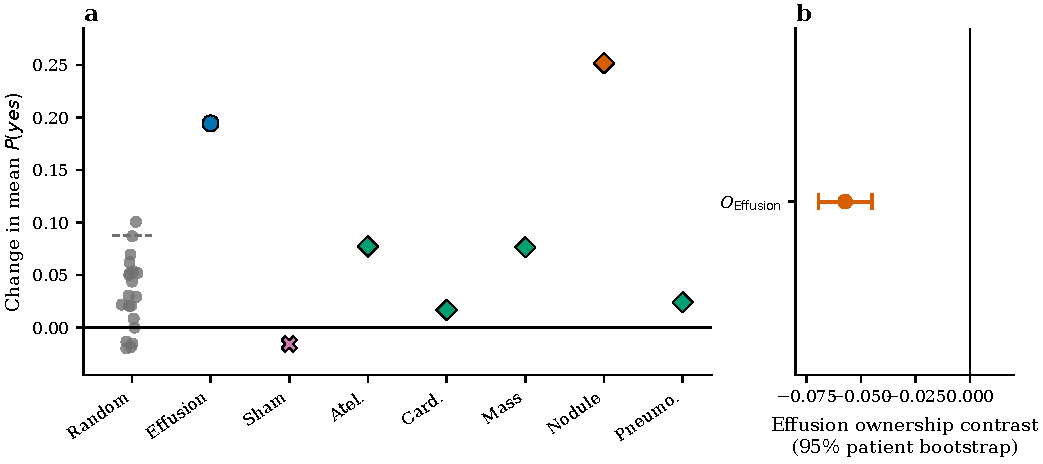
\includegraphics[width=0.90\textwidth]{figures/fig3_direction_specificity.pdf}
    \caption{\textbf{Qwen Effusion reproduces as a non-generic write direction, but semantic competition changes its attribution.} \textbf{(a)} Changes in mean $P(\mathrm{yes})$ at the locked dose $\alpha=+0.25$ on 400 patients absent from the original cohort. The random group contains 20 directions; its dashed segment marks p95. Diamonds show the five fixed alternative clinical normals. \textbf{(b)} The Effusion ownership contrast $O_{\mathrm{Effusion}}$ with its two-sided 95\% patient-bootstrap interval; the registered one-sided 95\% lower bound is $-0.0678$. Nodule realizes the point-estimate maximum.}
    \label{fig:specificity}
\end{figure}

\FloatBarrier

\subsection{Semantic competition changes attribution, not efficacy}
\label{sec:specificity-results}

The fixed clinical family provides a harder identification test than non-semantic controls. Nodule changes the Effusion answer by 0.2519 and realizes the point-estimate maximum among the five alternatives. The Effusion ownership contrast $O_{\mathrm{Effusion}}$ is $-0.0573$. Recomputing the maximum inside each of 5,000 patient-bootstrap draws gives a two-sided 95\% CI of $[-0.0694,-0.0450]$ and a one-sided 95\% lower bound of $-0.0678$. The entire interval is below zero. Descriptively, all five alternative clinical normals move the Effusion endpoint in the same positive direction; Effusion exceeds four by 0.1172--0.1778, while Nodule alone has a larger point estimate. This shared-sign pattern motivates an answer-sensitive-alias hypothesis but cannot distinguish it from question-specific ownership.

Qwen Effusion therefore remains a reproducible direction that changes the answer beyond random and sham perturbations, while its specific semantic attribution fails. The familywise endpoint establishes that at least one fixed clinical alternative is stronger; Nodule is the point-estimate maximizer, not a separately familywise-identified semantic owner.

\subsection{Prospective mechanism gates preserve the attribution boundary}
\label{sec:mechanism-results}

\begin{table}[!ht]
\centering
\caption{Prospective tests of clinical ownership, shared aliasing, and input closure in Qwen.}
\label{tab:mechanisms}
\resizebox{\ifdim\width>\linewidth\linewidth\else\width\fi}{!}{%
\begin{tabular}{llcccl}
\toprule
Gate & Cohort & \shortstack{Target \\ statistic} & \shortstack{Registered \\ comparator} & \shortstack{Uncertainty \\ boundary} & Outcome \\
\midrule
Ownership & 400 patients & Alias candidate 0.2909 & Random max 0.3402 & Alias LCB 0.2808 & 0/6 owned; no alias \\
Input closure & 50 pairs & Gain 0.0022 & Random max 0.0025 & \shortstack{Disp. LCB -0.0364; \\ clin. LCB -0.0015} & No closure \\
\bottomrule
\end{tabular}%
}
\end{table}


The causal-ownership matrix provides no named replacement for the failed Effusion attribution. All six diagonal ownership margins are negative, so zero of six clinical concepts is owned under the simultaneous and random-control rules. Every question column's strongest clinical direction is off-diagonal. Effusion is the strongest shared-alias candidate: its mean off-diagonal effect is 0.2909 with simultaneous lower bound 0.2808, and its relative-dominance lower bound is 0.1332. Yet the random alias maximum, taken over 119 directions and six five-question mean effects, is larger at 0.3402. The matrix therefore confirms neither clinical ownership nor a shared alias.

The Consolidation fallback separates availability from input closure on 50 fresh within-patient pairs. On the full patient-disjoint test split, its probe selectivity is 0.0642 with 95\% CI $[0.0302,0.0976]$, so the readout is eligible before pair selection. Across the 50 pairs, mean positive-minus-negative displacement along the Consolidation normal is 0.1091, but its one-sided lower bound is $-0.0364$. Writing the measured displacement back produces mean closure gain 0.0022, below the maximum over 119 random directions, 0.0025. The familywise Consolidation-minus-maximum-clinical lower bound is also negative at $-0.0015$. The input-closure conjunction is not met.

\begin{figure}[H]
    \centering
    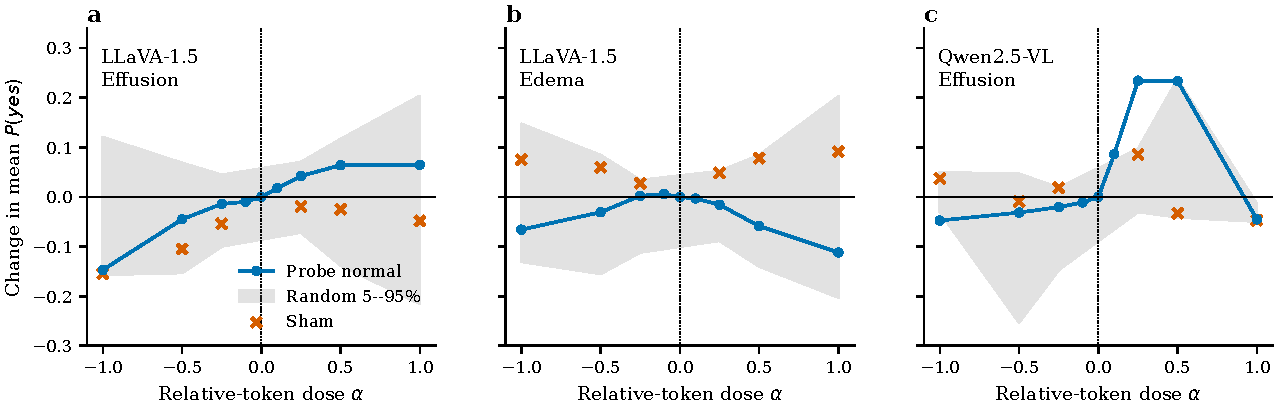
\includegraphics[width=\textwidth]{figures/fig2_dose_responses.pdf}
    \caption{\textbf{Comparable readers become different writers at the consumed final visual block.} The blue curve is the raw change in mean $P(\mathrm{yes})$ under the target probe normal on the same 200 held-out images per cell. Gray bands show the 5th--95th percentile across 20 equal-norm random directions at the six controlled nonzero doses; orange crosses show the coordinate-permutation sham. The concept-consistent rule uses $\operatorname{sign}(\alpha)\Delta(\alpha)$, accounting for the negative-dose maxima in the two LLaVA cells.}
    \label{fig:dose}
\end{figure}

\FloatBarrier

\subsection{The reader--writer mismatch begins earlier in LLaVA}
\label{sec:generic-results}

The LLaVA cells show that the mismatch can arise before semantic competition. Both are robust readers: Effusion reaches AUROC 0.7788 and selectivity 0.1139 (95\% CI $[0.0875,0.1404]$), while Edema reaches AUROC 0.8009 and selectivity 0.1360 ($[0.0994,0.1693]$). Their selectivity intervals exclude zero, as does Qwen's, but their write directions do not clear the registered random-and-sham conjunction (Figure~\ref{fig:dose}).

LLaVA Effusion attains a maximum concept-consistent change of 0.1470 at $\alpha=-1$. It exceeds the same-dose random p95 of 0.1202 but remains below the maximum absolute sham effect of 0.1546. Its monotone central response ($\rho=1.0$ over $[-0.5,0.5]$) is descriptively coherent, but does not distinguish the probe normal from the sham.

LLaVA Edema attains 0.0659 at $\alpha=-1$. It lies inside the same-dose random interval $[-0.1304,0.1470]$ and below the maximum absolute sham effect of 0.0913. Its descriptive dose monotonicity is $\rho=-0.4286$. Neither its random nor sham comparison supports a selective write effect.

The decoding contrasts reinforce this dissociation. Within LLaVA, Edema-minus-Effusion selectivity is 0.0221 with paired 95\% CI $[-0.0175,0.0590]$; for Effusion, Qwen-minus-LLaVA is 0.0026 with CI $[-0.0155,0.0215]$. The intervals do not resolve a reader ordering, while the generic-control outcomes still differ.

\subsection{Each control changes the scientific claim}

The experiments separate three statements that are often collapsed. Controlled decoding supports that a label is available to a fixed reader. Random and sham controls support that a labeled normal is an unusually effective writer relative to matched non-semantic perturbations. Semantic competition asks whether the clinical name attached by the reader is specific to that write effect. Qwen supports the first two statements but not the third; LLaVA establishes the first but not the second. Holding locus, dose, rows, endpoint, and uncertainty calculation fixed makes the reader--writer gap experimentally visible.

\begin{table}[H]
\centering
\scriptsize
\setlength{\tabcolsep}{3.2pt}
\caption{Intervention outcomes. Original cohorts maximize the concept-consistent effect over six fixed nonzero doses. The patient-disjoint cohort locks $\alpha=+0.25$; its registered fixed-family endpoint recomputes the maximum over five clinical alternatives inside each of 5,000 patient-bootstrap replicates. ``Supported interpretation'' states the strongest claim warranted by each cohort.}
\label{tab:gates}
\textit{Generic-control outcomes}\\[2pt]
\begin{tabular*}{\textwidth}{@{\extracolsep{\fill}}lllrrccc@{}}
\toprule
Model & Concept & Cohort & $N$ & $\alpha$ & Target $\Delta$ & Random 95th & $|$sham$|$ \\
\midrule
LLaVA-1.5-7B & Effusion & Original & 200 & -1.00 & 0.1470 & 0.1202 & 0.1546 \\
LLaVA-1.5-7B & Edema & Original & 200 & -1.00 & 0.0659 & 0.1470 & 0.0913 \\
Qwen2.5-VL-7B & Effusion & Original & 200 & +0.25 & 0.2343 & 0.0963 & 0.0852 \\
Qwen2.5-VL-7B & Effusion & Patient-disjoint & 400 & +0.25 & 0.1945 & 0.0878 & 0.0157 \\
\bottomrule
\end{tabular*}
\medskip

\textit{Fixed-family ownership outcome}\\[2pt]
\begin{tabular*}{\textwidth}{@{\extracolsep{\fill}}lllcl@{}}
\toprule
Model & Concept & Cohort & $O_{\mathrm{Effusion}}$ [95\% CI] & Supported interpretation \\
\midrule
Qwen2.5-VL-7B & Effusion & Patient-disjoint & -0.0573 [-0.0694, -0.0450] & Writer; Effusion ownership fails \\
\bottomrule
\end{tabular*}
\end{table}


Across the six gates, every target is available to the fixed readout, but generic selectivity, clinical specificity, ownership, aliasing, and input closure separate in turn. The ordered failures bound the concept-specific causal claim rather than erasing the underlying intervention effects.

\FloatBarrier
